% Options for packages loaded elsewhere
\PassOptionsToPackage{unicode}{hyperref}
\PassOptionsToPackage{hyphens}{url}
%
\documentclass[
]{article}
\usepackage{lmodern}
\usepackage{amssymb,amsmath}
\usepackage{ifxetex,ifluatex}
\ifnum 0\ifxetex 1\fi\ifluatex 1\fi=0 % if pdftex
  \usepackage[T1]{fontenc}
  \usepackage[utf8]{inputenc}
  \usepackage{textcomp} % provide euro and other symbols
\else % if luatex or xetex
  \usepackage{unicode-math}
  \defaultfontfeatures{Scale=MatchLowercase}
  \defaultfontfeatures[\rmfamily]{Ligatures=TeX,Scale=1}
\fi
% Use upquote if available, for straight quotes in verbatim environments
\IfFileExists{upquote.sty}{\usepackage{upquote}}{}
\IfFileExists{microtype.sty}{% use microtype if available
  \usepackage[]{microtype}
  \UseMicrotypeSet[protrusion]{basicmath} % disable protrusion for tt fonts
}{}
\makeatletter
\@ifundefined{KOMAClassName}{% if non-KOMA class
  \IfFileExists{parskip.sty}{%
    \usepackage{parskip}
  }{% else
    \setlength{\parindent}{0pt}
    \setlength{\parskip}{6pt plus 2pt minus 1pt}}
}{% if KOMA class
  \KOMAoptions{parskip=half}}
\makeatother
\usepackage{xcolor}
\IfFileExists{xurl.sty}{\usepackage{xurl}}{} % add URL line breaks if available
\IfFileExists{bookmark.sty}{\usepackage{bookmark}}{\usepackage{hyperref}}
\hypersetup{
  hidelinks,
  pdfcreator={LaTeX via pandoc}}
\urlstyle{same} % disable monospaced font for URLs
\usepackage{graphicx}
\makeatletter
\def\maxwidth{\ifdim\Gin@nat@width>\linewidth\linewidth\else\Gin@nat@width\fi}
\def\maxheight{\ifdim\Gin@nat@height>\textheight\textheight\else\Gin@nat@height\fi}
\makeatother
% Scale images if necessary, so that they will not overflow the page
% margins by default, and it is still possible to overwrite the defaults
% using explicit options in \includegraphics[width, height, ...]{}
\setkeys{Gin}{width=\maxwidth,height=\maxheight,keepaspectratio}
% Set default figure placement to htbp
\makeatletter
\def\fps@figure{htbp}
\makeatother
\setlength{\emergencystretch}{3em} % prevent overfull lines
\providecommand{\tightlist}{%
  \setlength{\itemsep}{0pt}\setlength{\parskip}{0pt}}
\setcounter{secnumdepth}{-\maxdimen} % remove section numbering

\author{}
\date{}

\begin{document}

\hypertarget{general-structure-of-an-os}{%
\section{General Structure of an OS}\label{general-structure-of-an-os}}

\hypertarget{separation-of-a-computer-in-four-sections}{%
\subsection{Separation of a computer in four
sections}\label{separation-of-a-computer-in-four-sections}}

\begin{itemize}
\item
  \textbf{Hardware :}

  collection of devices that allow the execution of programs
\item
  \textbf{OS :}

  management and coordination of system hardware
\item
  \textbf{Software :}

  any program that can be executed inside the OS
\item
  \textbf{User :}

  any device or being that can interact with the system
\end{itemize}

\hypertarget{hardware-simplified}{%
\subsection{Hardware (simplified)}\label{hardware-simplified}}

\begin{itemize}
\tightlist
\item
  Systembus connects all devices

  \begin{itemize}
  \tightlist
  \item
    one or more CPUs for program execution
  \item
    shared memory for tasks of the CPU and other devices
  \item
    Controller for IO devices

    \begin{itemize}
    \tightlist
    \item
      Hard Drives
    \item
      HID
    \item
      Network Interface
    \item
      \ldots{}
    \end{itemize}
  \end{itemize}
\end{itemize}

\begin{figure}
\centering
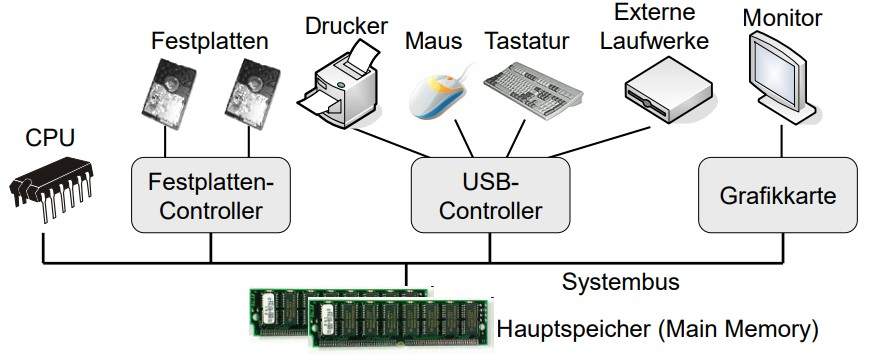
\includegraphics{images/BUS_Systembus-Flowchart.jpg}
\caption{``Systembus Floiwchart''}
\end{figure}

\hypertarget{computer-architecture-von-neumann}{%
\subsection{Computer Architecture :
von-Neumann}\label{computer-architecture-von-neumann}}

\begin{itemize}
\tightlist
\item
  reference model for computers
\item
  separation between code execution and data

  \begin{itemize}
  \tightlist
  \item
    Separation between CPU and memory
  \item
    Separation between Execution Unit and ALU
  \end{itemize}
\item
  this adds component communication overhead in program execution

  \begin{itemize}
  \tightlist
  \item
    Data has to be moved from memory to CPU and back, to be used
  \item
    the OS provides functionality to use the given resources efficiently
  \end{itemize}
\end{itemize}

\begin{figure}
\centering
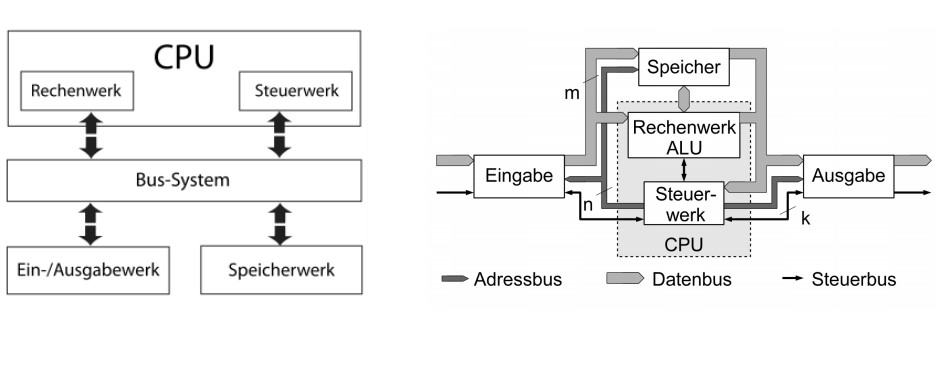
\includegraphics{images/CPU_model-flowchart.jpg}
\caption{``CPU Model Flowchart''}
\end{figure}

\begin{itemize}
\tightlist
\item
  CPU has multiple registers

  \begin{itemize}
  \tightlist
  \item
    data registers, address registers, special registers, \ldots{}
  \end{itemize}
\item
  additional cache

  \begin{itemize}
  \tightlist
  \item
    fast buffer memory
  \item
    access to cache is much faster compared to memory access
  \item
    smaller cache = lower access times
  \item
    caches are transparent to the OS
  \item
    Types of cache

    \begin{itemize}
    \tightlist
    \item
      L1-cache

      \begin{itemize}
      \tightlist
      \item
        close to the main execution unit, very small, very little
        latency
      \item
        saves future instructions for faste execution
      \end{itemize}
    \item
      L2-cache

      \begin{itemize}
      \tightlist
      \item
        larger and slightly slower
      \end{itemize}
    \item
      L3-cache

      \begin{itemize}
      \tightlist
      \item
        faster than main memory
      \item
        smaller than main memory
      \item
        extra chip outside the main processor
      \end{itemize}
    \end{itemize}

    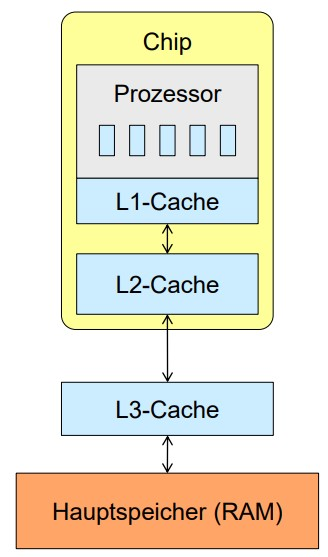
\includegraphics{images/CPU_registers-and-memory.jpg}
  \end{itemize}
\item
  registers tend to be very small, no more than the size of a DWORD but
  extremely fast

  \begin{itemize}
  \tightlist
  \item
    used for calculation or comparison
  \end{itemize}
\item
  cache is still very fast, but is usually slower than registers, while
  having a larger size
\item
  main memory is very large, but needs many cycles to move data to CPU

  \begin{itemize}
  \tightlist
  \item
    OS needs to handle access times and data transport
  \item
    every time we access data from a hard drive, we have to stop program
    execution so the processor can continue
  \end{itemize}
\end{itemize}

\hypertarget{processor-cores-and-caches}{%
\subsection{Processor Cores and
Caches}\label{processor-cores-and-caches}}

\begin{itemize}
\item
  each CPU tends to have its own L1 and L2 cache, sharing the L3 cache
  between all cores
\item
  all processors can access system BUS and main memory individually
\item
  communication and access latency is still a bottleneck in modern
  hardware
\item
  Hyperthreading

  \begin{itemize}
  \tightlist
  \item
    process interweaving, so that program execution can be sped up
  \end{itemize}
\end{itemize}

\hypertarget{hardware-component-interplay}{%
\subsection{Hardware component
interplay}\label{hardware-component-interplay}}

\begin{itemize}
\tightlist
\item
  CPU executes operations
\item
  CPU and IO-devices are used asynchronously

  \begin{itemize}
  \tightlist
  \item
    every IO-controller controls one type of device
  \item
    the CPU is needed to execute an operation

    \begin{itemize}
    \tightlist
    \item
      every controller has its own registers
    \item
      CPU moves data from main memory and cache
    \item
      operation is started after moving the data
    \end{itemize}
  \item
    Today: \emph{DMA (Direct Memory Access)}

    \begin{itemize}
    \tightlist
    \item
      seperate controller for the movement of data
    \item
      takes load away from CPU
    \end{itemize}
  \end{itemize}
\end{itemize}

\hypertarget{simplified-computer-architecture}{%
\subsection{Simplified computer
architecture}\label{simplified-computer-architecture}}

\begin{figure}
\centering
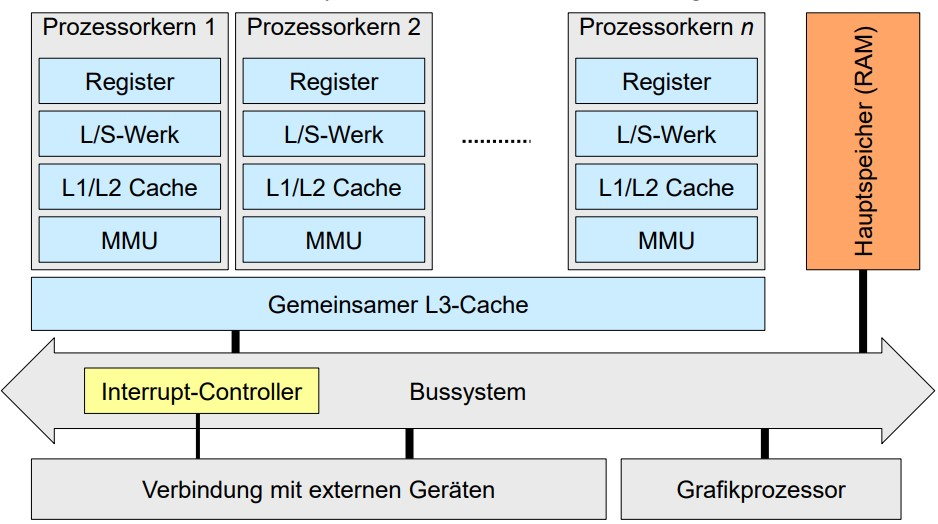
\includegraphics{images/Computer_Arch_Simplified.jpg}
\caption{``Main Components of a computer''}
\end{figure}

\end{document}
